\documentclass[14pt, unknownkeysallowed]{beamer}
\usepackage{tikz}
\usepackage{comment}
\usepackage{fancyvrb}
\usepackage{tikz}
\usetikzlibrary{arrows,decorations.pathmorphing,backgrounds,positioning,fit,petri}
\usepackage{hyperref}

\usepackage[default]{berasans}
\renewcommand*\familydefault{\sfdefault}  %% Only if the base font of the document is to be sans serif
\usepackage[T1]{fontenc}

\setbeamertemplate{navigation symbols}{}
\usetheme{Dresden}
\usecolortheme{seagull}
\usefonttheme{professionalfonts}


\title{Using Simpy to Model the Restoration of the Puerto Rican Power Grid}
\author{Thad Haines}
\institute[CSCI 577]{Montana Tech - CSCI 577 - 2018 Term Project}
\date{December 13, 2018}

\begin{document}

\begin{frame}
\titlepage
\end{frame}

%************************************************
\section{Introduction}
%------------------------------------------------
\subsection{Quick Background Information}
\begin{frame}
\frametitle{Puerto Rico is an Island}
\framesubtitle{3,515 mi$^{2}$ land area;
\end{frame}
%------------------------------------------------
\subsection{Problem Statement}
\begin{frame}
\frametitle{Puerto Rico is an Island}
\framesubtitle{Hurricanes can damage Power Transmission Systems}
Problem Statement:
\begin{itemize}
	\item Hurricane Maria damaged 80\% of the Puerto Rican power system.
	\item It took 9 months to restore $\approx$99\%.
	\item Access to supplies and workers may have affected the time required.
\end{itemize}
\end{frame}
%------------------------------------------------
\begin{frame}
\begin{block}{Goal}
Create a DEDS model that mimics the known restoration of the Puerto Rican
power system using Simpy.
\end{block}
\begin{block}{Thesis Question}
	Would more available resources speed up the restoration process? If so, how much?
\end{block}
\end{frame}

%************************************************
\section{SUI}
%------------------------------------------------
\subsection{Overview}
\begin{frame}
\frametitle{Basic System}
\begin{itemize}
	\item Supplies generated and collected at Mainland HQ.
	\item Supplies sent from Mainland HQ to Island HQ via Ship.
	\item Workers move between HQs via Plane.
	\item Island HQ applies Work Hours and Supplies to Power System.
\end{itemize}
\end{frame}
%------------------------------------------------


%************************************************
\section{Conceptual Model}
%------------------------------------------------
\subsection{Entities}
\begin{frame}
\frametitle{Simulation Objects}
\framesubtitle{All objects could be thought of as Resources and Consumers}
\begin{itemize}
	\item Mainland HQ
	\item Island HQ
	\item Power System
	\item Ship (transient)
	\item Watchdog (log)
\end{itemize}
\end{frame}
%------------------------------------------------
\begin{frame}
\frametitle{Simulation Resources}
\framesubtitle{'Most' resources begin at mainland HQ and move to island HQ.}
\begin{itemize}
	\item Wire
	\item Poles
	\item Workers (Used as Work Hours)
	\item Ships
	\item Power System Wire and Pole Status
\end{itemize}
\end{frame}
%------------------------------------------------
\begin{frame}
\frametitle{Model Environment}
\framesubtitle{Default simpy.Enivronment()}
\begin{itemize}
	\item Time step in days
	\item All other objects 'attached' to environment for 'ease' of use and data collection.
\end{itemize}
\end{frame}
%------------------------------------------------
\subsection{State Charts}
%------------------------------------------------
\begin{frame}
\frametitle{Resource Flow}
yup
\end{frame}

%************************************************
\section{Testing}
%------------------------------------------------
\subsection{Double Island Workers Case Results}
%_______________________________
\begin{frame}
Total Restoration
\begin{figure}
	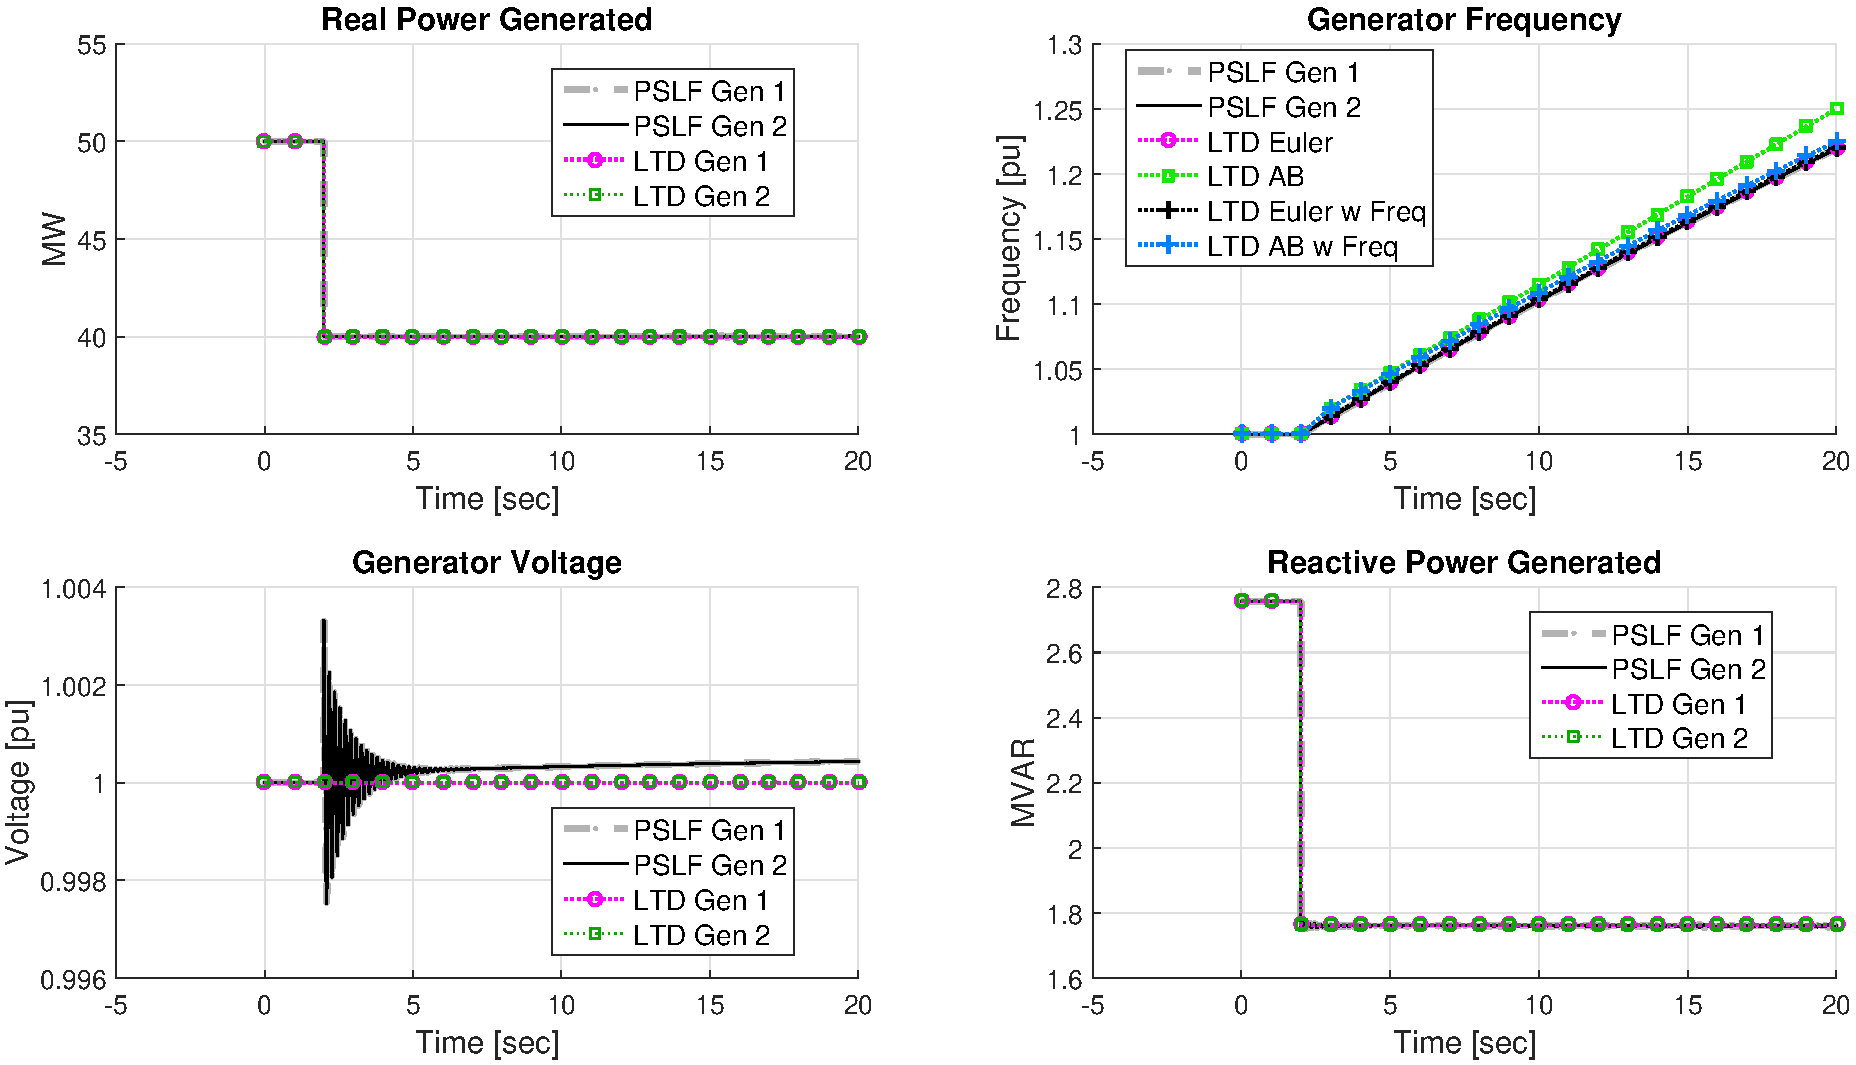
\includegraphics[width=\linewidth]{noGovExcLoadStepDsys}
\end{figure}
\end{frame}

%************************************************
\section{Conclusion}
%------------------------------------------------
\begin{frame}
\begin{itemize}
	\item Model suggests more resources (workers especially) will speed up restoration.
	\item Maximum speedup around 90 days.
	\item Model probably too simple for situation.
	\item More known data required for proper simulation.
\end{itemize}
\end{frame}
%------------------------------------------------
\subsection{References}
\begin{frame}
\resizebox{.8\textwidth}{.4\textheight}{
\begin{minipage}{\textwidth}
	\begin{itemize}
	\item[[1]] https://spectrum.ieee.org/energy/policy/rebuilding-puerto-ricos-power-grid-the-inside-story
	\item[[2]] https://www.economist.com/united-states/2017/10/19/the-story-of-puerto-ricos-power-grid-is-the-story-of-puerto-rico
	\item[[3]] https://twitter.com/AEEONLINE/status/1006493557908279297/photo/1
	\item[[4]] https://www.nytimes.com/2018/08/14/us/puerto-rico-electricity-power.html
\end{itemize}
\end{minipage}
}
\end{frame}

\end{document}